\usetikzlibrary {automata,positioning}
\scalebox{0.9}{
    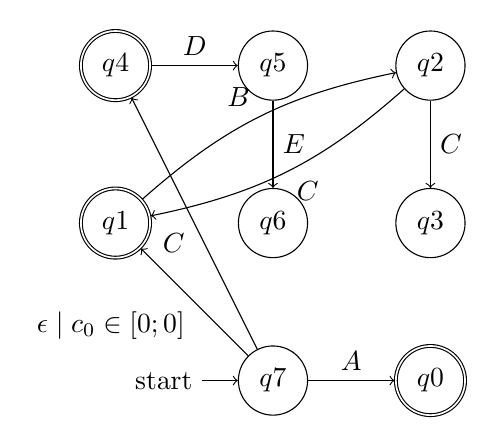
\begin{tikzpicture}[auto]
        \node[state, accepting] at (0, 0)(q4){$q4$};
        \node[state] at (2, 0)(q5){$q5$};
        \node[state] at (2, -2)(q6){$q6$};
        \node[state, accepting] at (0, -2)(q1){$q1$};
        \node[state] at (4, 0)(q2){$q2$};
        \node[state] at (4, -2)(q3){$q3$};
        \node[state, accepting] at (4, -4)(q0){$q0$};
        \node[state, initial] at (2, -4)(q7){$q7$};

        \path[->]
        (q2)edge node{$C$}(q3)
        (q1)edge [bend left=15] node{$B$}(q2)
        (q2)edge [bend left=15] node{$C$}(q1)
        (q5)edge node{$E$}(q6)
        (q4)edge node{$D$}(q5)
        (q7)edge node{$A$}(q0)
        (q7)edge node{$\epsilon\mid c_0\in[0;0]$}(q1)
        (q7)edge node{$C$}(q4)
        ;
    \end{tikzpicture}
}
\captionof{figure}{TA with UPPAALs state positioning.}
\label{fig:uppaalLayout}